\documentclass[arhiv]{../izpit}
\usepackage{fouriernc}
\usepackage{xcolor}
\usepackage{tikz}

\begin{document}

\izpit{Programiranje I: 1.\ izpit}{24.\ januar 2018}{
  Čas reševanja je 180 minut.

  \textbf{Naloge 1, 2 in 3 rešite v OCaml-u, nalogo 4 pa lahko rešite v
  OCaml-u ali Python-u.}

  Veliko uspeha!
}

%%%%%%%%%%%%%%%%%%%%%%%%%%%%%%%%%%%%%%%%%%%%%%%%%%%%%%%%%%%%%%%%%%%%%%
\naloga[]

\podnaloga
  Definirajte funkcijo \texttt{print\_all}, ki sprejme seznam celih števil,
  zaporedoma izpiše vse elemente seznama in vrne \texttt{unit}.

  \begin{verbatim}
    print_all [1; 2; 3; 4];;
    1234- : unit = ()
  \end{verbatim}

\podnaloga
  Definirajte funkcijo \texttt{map2\_opt}, ki sprejme dva seznama in funkcijo
  dveh argumentov. Vrne naj seznam rezultatov, ko dano funkcijo zaporedoma
  uporabimo na isto ležečih elementih seznamov. Želimo, da funkcija deluje zgolj
  kadar sta oba vhodna seznama enake dolžine, zato uporabite tip \texttt{option}.

  Za maksimalno število točk naj bo funkcija repno rekurzivna.

  \begin{verbatim}
    # map2_opt [1; 2; 3] [7; 5; 3] (+);;
    - : int list option = Some [8; 7; 6]
  \end{verbatim}


%%%%%%%%%%%%%%%%%%%%%%%%%%%%%%%%%%%%%%%%%%%%%%%%%%%%%%%%%%%%%%%%%%%%%%
\naloga[]

Filtracijsko drevo ima dve vrsti osnovnih gradnikov:
\begin{itemize}
\item Vozlišča imajo celoštevilsko vrednost, levo poddrevo in desno poddrevo.
\item Listi oz. škatle imajo seznam celoštevilskih vrednosti.
\end{itemize}

\noindent Primer \texttt{test\_tree}:
\[
  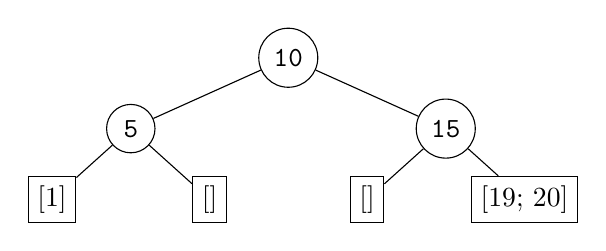
\begin{tikzpicture}[level distance=0.9cm,
    level 1/.style={sibling distance=4cm},
    level 2/.style={sibling distance=2cm},
    level 3/.style={sibling distance=2cm}
    ]
    \node[circle, draw] {\texttt{10}}
      child {node[circle, draw] {\texttt{5}}
        child {node[rectangle, draw] {[1]}}
        child {node[rectangle, draw] {[]}}
      }
      child {node[circle, draw] {\texttt{15}}
        child {node[rectangle, draw] {[]}}
        child {node[rectangle, draw] {[19; 20]}}
      };
  \end{tikzpicture}
\]

\podnaloga
  Definirajte tip \texttt{filter\_tree}, ki predstavlja filtracijsko drevo in
  nato konstruirajte zgornji primer \texttt{test\_tree}.

\podnaloga
  Filtracijsko drevo razvršča števila v škatle glede na njihovo vrednost.
  Vozlišče z vrednostjo $k$ razvrsti število $n$ v levo poddrevo če velja
  $n \leq k$ oz.\ v desno poddrevo če velja $n > k$.
  Ko število doseže škatlo, ga dodamo v seznam števil v škatli.
  Škatle lahko vsebujejo ponovitve in niso nujno urejene.

  Napišite funkcijo \texttt{insert}, ki sprejme število in filtracijsko drevo in
  vrne filtracijsko drevo z vstavljenim številom.

  \begin{verbatim}
    # insert 12 test_tree;;
  \end{verbatim}
  \[
    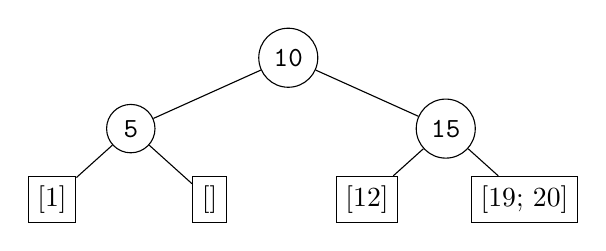
\begin{tikzpicture}[level distance=0.9cm,
      level 1/.style={sibling distance=4cm},
      level 2/.style={sibling distance=2cm},
      level 3/.style={sibling distance=2cm}
      ]
      \node[circle, draw] {\texttt{10}}
        child {node[circle, draw] {\texttt{5}}
          child {node[rectangle, draw] {[1]}}
          child {node[rectangle, draw] {[]}}
        }
        child {node[circle, draw] {\texttt{15}}
          child {node[rectangle, draw] {[12]}}
          child {node[rectangle, draw] {[19; 20]}}
        };
    \end{tikzpicture}
  \]

\podnaloga
  Napišite funkcijo \texttt{insert\_many}, ki sprejem seznam celih števil in
  filtracijsko drevo ter vrne filtracijsko drevo z vstavljenimi elementi seznama.
  Vrstni red vstavljanja ni pomemben.

\podnaloga
  Definirajte funkcijo, ki sprejme filtracijsko drevo in preveri ali
  so vsa števila v pravilnih škatlah glede na način razvrščanja.

  \[
    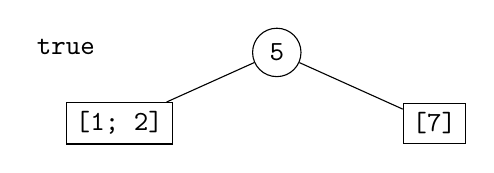
\begin{tikzpicture}[level distance=0.9cm,
      level 1/.style={sibling distance=4cm},
      level 2/.style={sibling distance=2cm}
      ]
      \node[circle, draw] {\texttt{5}}
        child {node[rectangle, draw] {\texttt{[1; 2]}}}
        child {node[rectangle, draw] {\texttt{[7]}}};

      \node[align=left,yshift=5mm] at (current bounding box.west) {\texttt{true}};
    \end{tikzpicture}
    \hspace{15mm}
    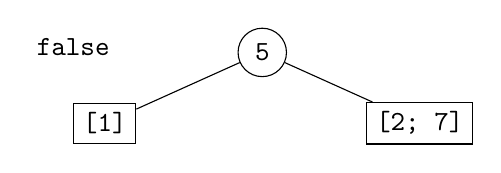
\begin{tikzpicture}[level distance=0.9cm,
      level 1/.style={sibling distance=4cm},
      level 2/.style={sibling distance=2cm}
      ]
      \node[circle, draw] {\texttt{5}}
        child {node[rectangle, draw] {\texttt{[1]}}}
        child {node[rectangle, draw] {\texttt{[2; 7]}}};

      \node[align=left,yshift=5mm] at (current bounding box.west) {\texttt{false}};
    \end{tikzpicture}
  \]

%%%%%%%%%%%%%%%%%%%%%%%%%%%%%%%%%%%%%%%%%%%%%%%%%%%%%%%%%%%%%%%%%%%%%%
\naloga[]
Linearne preslikave na vektorjih lahko predstavimo tako s funkcijami kot z
matrikami.
Vektorje in matrike bomo tokrat predstavljali s pari oz.\ četvorci.

\[
\begin{bmatrix}
    x\\
    y
\end{bmatrix}
=
(x, y)
\hspace{5mm}
\begin{bmatrix}
    a & b \\
    c & d
\end{bmatrix}
=
(a, b, c, d)
\]

V datoteki \texttt{naloga3.ml} se nahaja že napisana signatura modula,
s katerim predstavimo linearne preslikave.

Signatura \texttt{Linear} določa:
\begin{itemize}
\item \texttt{t}: osnovni tip modula.
\item \texttt{id}: identiteta.
\item \texttt{apply}: sprejme vektor in preslikavo tipa \texttt{t} in uporabi preslikavo na vektorju.
\item \texttt{of\_matrix}: sprejme matriko in jo pretvori v tip \texttt{t}.
\item \texttt{of\_function}: sprejme linearno preslikavo in jo pretvori v tip \texttt{t}.
\item \texttt{compose}: sprejme dve preslikavi tipa \texttt{t} in vrne njun kompozitum.
\end{itemize}

\podnaloga
  Napišite modul \texttt{Matrix}, ki za predstavitev linearnih preslikav
  uporablja matrike.

\podnaloga
  Napišite modul \texttt{Function}, ki za predstavitev linearnih preslikav
  uporablja funkcije.

%%%%%%%%%%%%%%%%%%%%%%%%%%%%%%%%%%%%%%%%%%%%%%%%%%%%%%%%%%%%%%%%%%%%%%
\naloga[]

Lisjaček krade jabolka v sadovnjaku, kjer so jablane razporejene v vrstah.
Okrade lahko zgolj $N$ jablan preden ga prežene lastnik sadovnjaka.

Ker je lisjaček še mlad in nevešč kraje jabolk, v vsaki vrsti obira
jablane eno za drugo in pri tem nobene ne preskoči. Ko se odloči, da se bo
lotil naslednje vrste se ne vrne več nazaj. V primeru, da se znajde na koncu
zadnje vrste svojo avanturo zaključi, ne glede na to ali ima na voljo še kakšno
obiranje.

\podnaloga
  Napišite algoritem, ki izračuna največje število jabolk, ki jih lisjaček
  lahko ukrade. Sadovnjak predstavimo z matriko, kjer vrste predstavljajo
  vrste sadovnjaka in vrednosti v matriki število jabolk na jablani.
  V smislu matrike se lahko lisjaček premika zgolj v desno ali pa na začetek
  nove vrstice, kjer za vsak premik porabi en korak.

  \[
  {\texttt{N}}
  =
  6,
  \hspace{5mm}
  {\texttt{sadovnjak}}
  =
  \begin{bmatrix}
      1 & 2 & 0 & 5 \\
      0 & 4 & 1 & 1 \\
      8 & 0 & 4 & 2
  \end{bmatrix}
  \hspace{5mm}
  \mapsto
  \hspace{5mm}
  17
  \]

  Za vse točke mora biti funkcija učinkovita (ne eksponentna časovna
  zahtevnost).

  \podnaloga
  V komentarju napišite in utemeljite kakšna je časovna zahtevnost vašega algoritma.

\end{document}
